% CREATED BY DAVID FRISK, 2016
\chapter{Results}
\todo{Write something suitable here}These are the results!!!
%

\section{Sample case. Kleinmaterial: Nätverk}
Each teaching material tested has a different story to tell. Keep in mind that some of the content of the steps below are common to all teaching materials tested and some are original to the particular teaching material.

\subsection{The preexisting work}
The sample teaching material...
\begin{description}
    \item $\bullet$ ...had been produced by a team, consisting of a handful of teachers, a subject expert and a Klein-representative.
    \item $\bullet$ ...was published on Kleindagarna's website.
\end{description}

\subsection{Usability test I}
This first usability test was performed by one of the authors of this report on the other author, primarily to identify what to take into account for future usability testing and to identify the possibility of improving the usability testing methodology. The methodology consisted of a document on a computer including a table made to be filled with personal information and a list of keywords and questions (manuscript) inspired by the usability test script created by Steve Krug. Results from this test included:
\begin{description}
    \item $\bullet$ Unclear if some tasks are meant to be executed by teacher or students.
    \item $\bullet$ The material, maybe involuntarily, expect the teacher to be very familiar with the subject, tackling advanced areas of mathematics with mostly bullet points, expecting the teacher to provide the explanation.
    \item $\bullet$ There is a concern on the material having too large scope. The material includes network theory, statistics, algorithms and data protection laws (GDPR), and aims to both explain and problematize all of these aspects.
\end{description}
\subsection{Revision of methodology}
After usability testing the teaching material, the authors identified that there was very limited information presented in the list of teaching materials on Kleindagarna's website. This made it difficult for the curious to know if the material was suitable for them. Because of that, a new list of teaching materials was compiled. This consisted of information not just what the subject of the material was, but also for what grade it was suited and a more detailed description of the teaching material.\\
Another feature discussed after the usability test was whether teaching materials should be revised as a document solely intended as a foundation that a teacher later could build a lesson around or if revisions instead should design the teaching materials as ready-made presentations, giving the teacher a choice to use it as-is, altering it or just using it as inspiration. The discussion culminated in the decision to decide on a case-by-case basis, considering factors such as results from usability tests, perceived intent of original creators and what form would be most suited to the particular teaching material.
\subsection{Watching the Klein-lecture}
Before designing a teaching material, the participators on Kleindagarna receive a lecture by the subject-expert. This lecture was recorded and confidentially shared online. Before revising the material, it was decided that it would be beneficial to watch this lecture, to learn more about the theory the material was based upon and what the creators intended the students would learn.
\subsection{Usability test II}
The same revision was tested again. The test subject this time was a Klein-representative that had been involved in the creation of the original teaching material. Testing teaching materials on a subject that was not a teacher in upper-secondary-school or a teacher student aiming to teach at upper-secondary-school was not the norm. One purpose of this was to analyze how rewarding usability testing non-intended subject could be. The test subject is also teaching mathematics on an upper-secondary-school level, but to post-secondary school students (one additional difference is that the pace of the courses are comparably higher than in upper-secondary-school). Results from this test included:
\begin{description}
    \item $\bullet$ The teaching material wasn't considered complete by the creators.
    \item $\bullet$ The biggest remaining problem of the material design lies in a student activity where the class are to compile data to create a network. To be able to make the network and its analysis meaningful, it was suggested that the compiled data should be personal and able to lead to a finding. Ultimately, the activity asks for generated data, instead of personal, more valuable data. The reason for this is because no conceivable alternative could eliminate the risk that personal data could result in undesirable findings. For example if the data collected answers what students had lunch together, outcasts are visible in the finding.
    %\item $\bullet$
\end{description}
\subsection{Revision of teaching material}
From the data collected, the following revisions were made:
A decision was made to revise the material in the form of a presentation. With the aim to offer a ready-made presentation with enough explanation of the required theory to be a desirable product. To realize this, changes were made to the structure and to content.
\subsubsection*{Structural changes}
\begin{description}
    \item $\bullet$ The separation of information to the teacher and the main presentation was improved by implementing tabs similar to how many websites function. This also clarified the structure to the user, enabling the user to quickly get an overview of the structure.
    \item $\bullet$ The presentation's first slides contains useful information targeted to a curious teacher including how to read the important presentation notes (as these consists of teacher instructions and explanations).
\end{description}
\subsubsection*{Content changes}
\begin{description}
    \item $\bullet$ As mentioned previously, the presentation contains teacher instructions and explanations in the form of presentation notes. These can be printed or read in the presentation program, and also viewed while presenting. This was previously missing from the teacher material, or carelessly intertwined with content that seemed to be aimed to students.
    \item $\bullet$ Activities were altered to be either less vague or more closely tied to what the students are expected to learn.
    \item $\bullet$ The content was modified to be easily understood and conveyed. An example of this was replacing the headings so that they describe their respective slide, instead of being named after the current 5E-phase.
\end{description}
\subsection{What was learned from this case?}
From this particular case, the following knowledge was obtained:
\begin{description}
    \item $\bullet$ Someone involved in the creation of a teaching material can have a very different experience and connection to the teaching material, than is conveyed to a reader. Maybe there's a part the creator is not satisfied with, but the reader might assume it is meant to be complete and only understand it as poorly made. This exemplifies the flaws of one-way communication perfectly.
    \item $\bullet$ There needs to be a decision on how the teaching material is presented and what it aims to be. It can be everything from inspiring reading material to a documentary. It was decided that the two types of material explored in this thesis would be \textit{document with proposed lesson plan} and \textit{ready-made presentation}.
\end{description}

\section{The materials list}
\begin{figure}[H]
\centering
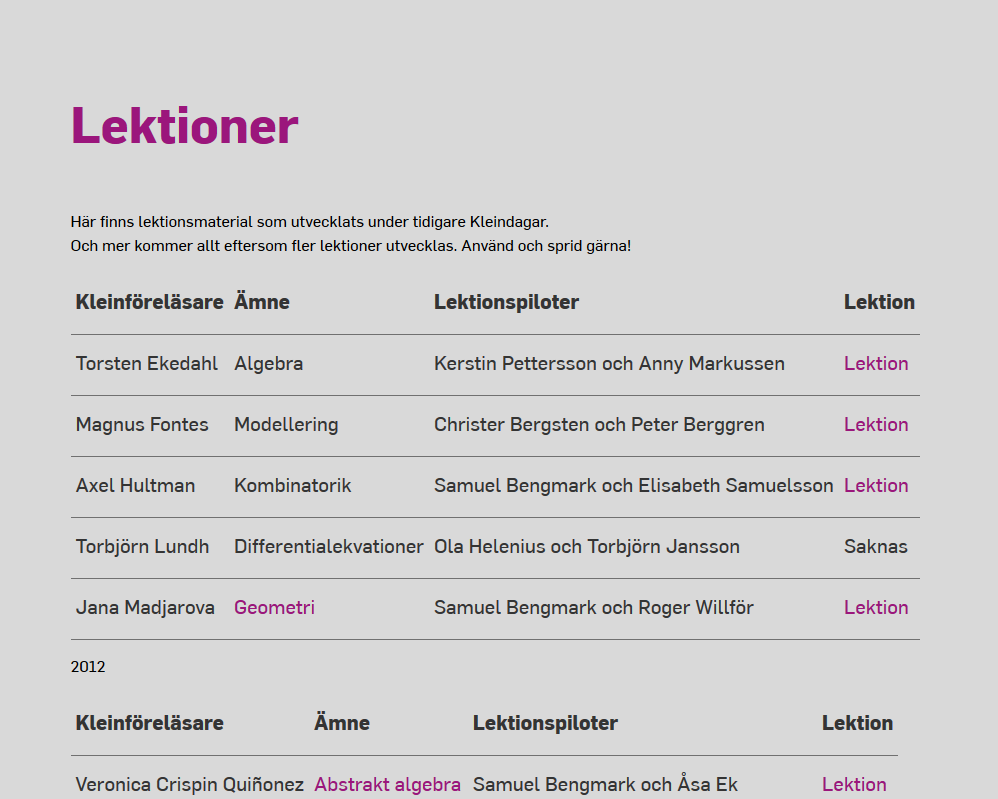
\includegraphics[width=\linewidth]{figure/screenshot_materiallista_kleindagarna.png}
\caption{The original list of materials on Kleindagarna's official website [SOURCE].}
\end{figure}

It is important to note that the design of Kleindagarna's list of materials changed in the middle of the thesis. Most of the information in the list remained the same, but colors and fonts changed. A screenshot of the list before Kleindagarna's change wasn't made and thus the exact changes were lost. The first and second thesis-revisions of the list were made before Kleindagarna made changes to their list.

\begin{figure}[H]
\centering
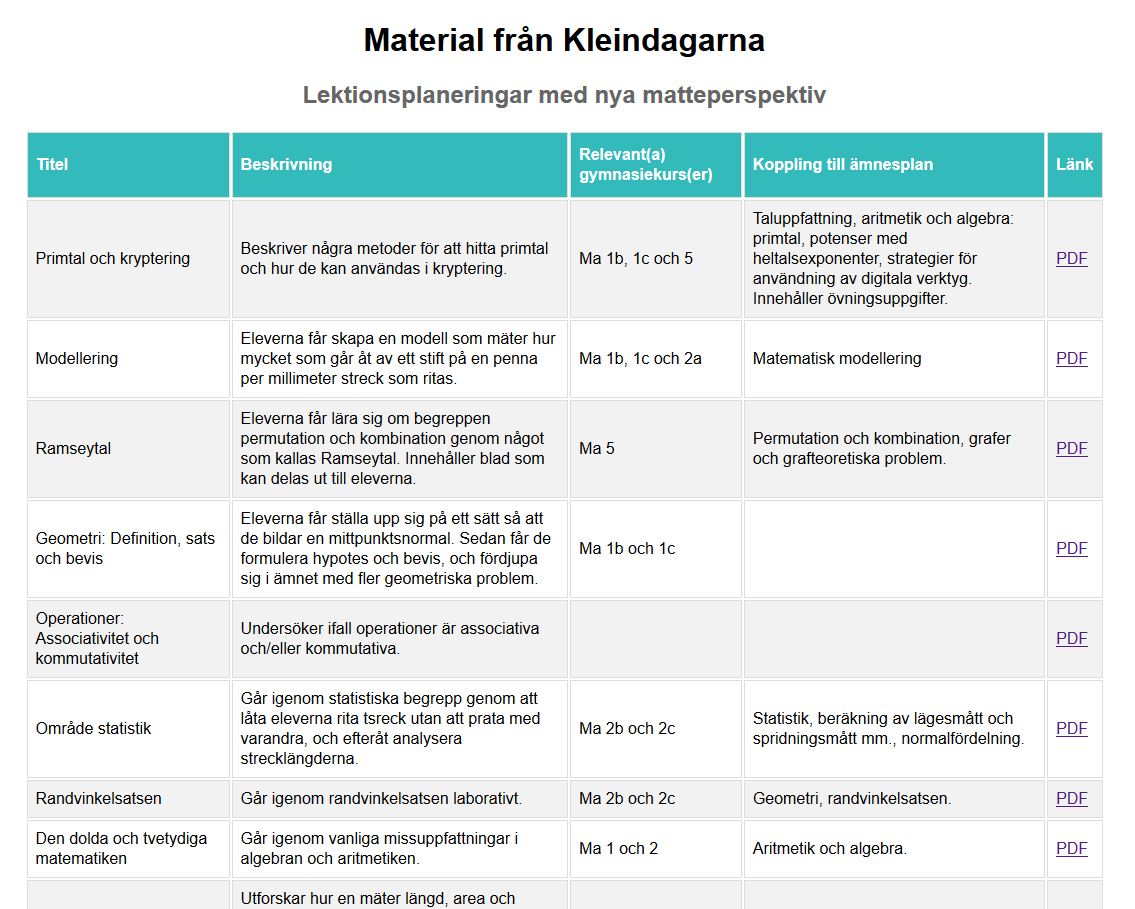
\includegraphics[width=\linewidth]{figure/screenshot_materiallista_revision_2.png}
\caption{The second revision of the list of materials, based on Kleindagarna's original [FIGURE REFERENCE?].}
\end{figure}
